\section{Parameterization of model titration} 
% - Jack/Ruibin
CpHMD is a relative free energy simulation approach, whereby the potential of mean force (PMF) of deprotonation of
a titratable amino acid in the protein environment is calculated relative to that of a reference, i.e., a model compound or peptide in solution
\cite{Lee_Brooks_2004_Proteins,Khandogin_Brooks_2005_Biophys.J.}. 
Model compounds, which were used in the early development of CpHMD methods
\cite{Lee_Brooks_2004_Proteins,Khandogin_Brooks_2005_Biophys.J.,Huang_Shen_2016_J.Chem.TheoryComput.},
are blocked single amino acid residues \ce{CH3CO}-X-\ce{NH2} or \ce{CH3CO}-X-\ce{CONH2},
where X represents a titratable amino acid.
In the development of the hybrid-solvent CpHMD \cite{Wallace_Shen_2011_J.Chem.TheoryComput.} and GBNeck2-CpHMD \cite{Huang_Shen_2018_J.Chem.Inf.Model.,Harris_Shen_2019_J.Chem.Inf.Model.}, 
model peptides 
\ce{CH3CO}-AAXAA-\ce{NH2} were used to take advantage of recent experimental data \cite{Thurlkill_Pace_2006_ProteinSci.,Platzer_McIntosh_2014_J.Biomol.NMR}.
Since in the CpHMD simulation, a model PMF is subtracted,
simulation of a model compound or peptide should return a zero PMF at the pH value equal to the model {\pka}.
In other words, protonated and deprotonated states are sampled with equal probabilities ($S\approx0.5$).
To ensure this is the case, the model PMF needs to be accurately determined.

To obtain the model PMF $U^{\rm mod}$, we use a free energy 
simulation method called thermodynamics integration,
in which the mean forces at different values of $\theta$ (for single site titration)
or $\theta$ and $x$ for double site titration
% $\langle\partial U/\partial\theta|_{\theta_i}\rangle$,
are calculated and then analytically
integrated to obtain $U^{\rm mod}$.
The single site titration model is applied
to Cys and Lys. The latter has equivalent protons, so one is selected for titration.
There are two types of double site titration model. His sidechains have two titratable nitrogens with different microscopic {\pka's}, while
carboxylate sidechains (Asp and Glu) have two titratable oxygens but identical microscopic {\pka's}.
These three titration models require
different forms of $U^{\rm mod}$ and methods of fitting.

\subsection{Protocol of parameterization for single site model titration}
For running TI simulations to obtain parameters, we set the options \textbf{prlam} to FALSE, \textbf{prderiv} to TRUE, and \textbf{phtest} to TRUE in the phmdin file, vph{\_}theta to 0 in the phmdstrt file.
For a single site titration model (e.g., Cys and Lys), 
we run CpHMD simulations at
$\theta_i=\left(0.4,0.6,0.785,1.0,1.2,1.4\right)$.
Each simulation is run for 10 ns, from which the mean forces
$\langle\partial U/\partial\theta|_{\theta_i}\rangle$
are calculated. 
Fitting of the mean forces  
to the following analytic form of $\partial U/\partial\theta$ (Eq.~\ref{Eq:dU_dtheta}) returns the two parameters $A$ and $B$ (Fig.~\ref{Fig:parm_cys}).

\begin{equation}
    \frac{\partial U}{\partial\theta}=2A\sin\left(2\theta\right)\left(\sin^{2}\theta-B\right).
    \label{Eq:dU_dtheta}
\end{equation}
As an example, Fig.~\ref{Fig:parm_cys} shows the fitting result for the GBNeck2-CpHMD titration of  Cys model peptide.
We note, fitting should be performed in the $\theta$ space (and not $\lambda$ space) to reduce errors.
 %--------------------------------------------- 
\begin{figure}[htb!]
    \centering
    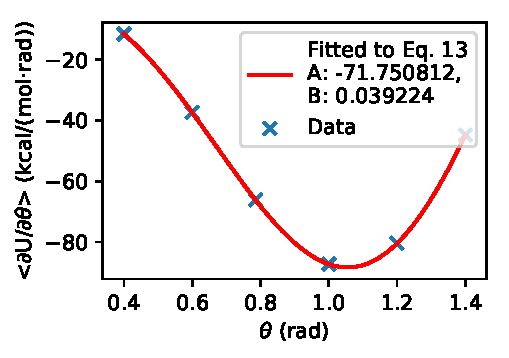
\includegraphics[width=3.3in]{figs/cys_parm.pdf}
    \caption{\textbf{Example of fitting A and B parameters for a single site titration model.}
    }
\label{Fig:parm_cys}
\end{figure}
 %--------------------------------------------- 

\paragraph{Protocol of parameterization for histidine model titration}
For a double site titration model 
with two different microscopic \pka's
(e.g. His), the two-dimensional PMF (Eq.~\ref{eq:double}) can be reduced to the
following form
\cite{Khandogin_Brooks_2005_Biophys.J.},

\begin{align}
U^{\rm mod}= & A_{10}\lambda^{2}x^{2}+2\left(A_{1}B_{1}-A_{0}B_{0}\right)\lambda x \nonumber \\ & + 2\left(A_{0}B_{0}-A_{1}B_{1}-A_{10}B_{10}\right)\lambda^{2}x \nonumber \\ & + A_{1}\lambda^{2}-2A_{1}B_{1}\lambda,
\label{eq:PMF_his}
\end{align}
where $\lambda=sin^2\theta$ and $x=sin^2\theta^x$. 
The six parameters $A_{0}$, $B_{0}$, $A_{1}$,  $B_{1}$, $A_{10}$, and $B_{10}$ are the parameters
in the quadratic functions
that describe the one-dimensional processes
\cite{Khandogin_Brooks_2005_Biophys.J.}.
$A_0$ and $B_0$ correspond to \ce{HIP <=> HID},
i.e., titration at N$\epsilon$;
$A_1$ and $B_1$ correspond to \ce{HIP <=> HIE},
i.e., titration at N$\delta$;
and $A_{10}$ and $B_{10}$ correspond to the tautomer interconversion \ce{HIE <=> HID}.


\textbf{Step 1.}
To obtain $A_0$ and $B_0$, we 
run TI simulations by fixing
$\theta^{x}$ at 0 ($\lambda=0$, HID, N$\delta$ is protonated), varying
$\theta$ at $\left(0.0,0.2,0.4,0.6,\\
0.785,1.0,1.2,1.4,1.5708\right)$, and fitting
the resulting mean forces to the following one-dimensional function,
\begin{equation}
    \frac{\partial U}{\partial\theta}=2A_{0}\sin\left(2\theta\right)\left(\sin^{2}\theta-B_{0}\right).
\end{equation}

\textbf{Step 2.}
To obtain $A_1$ and $B_1$,
we run TI simulations by fixing
$\theta^{x}$ at 1.5708 ($\lambda=1$, HIE, N$\delta$ is protonated), varying
$\theta$ at $\left(0.0,0.2,0.4,0.6,\\
0.785,1.0,1.2,1.4,1.5708\right)$, and 
fitting
 to the following one-dimensional function,
\begin{equation}
    \frac{\partial U}{\partial\theta}=2A_{1}\sin\left(2\theta\right)\left(\sin^{2}\theta-B_{1}\right).
\end{equation}

\textbf{Step 3.}
To obtain $A_{10}$ and $B_{10}$, we run TI simulations by fixing $\theta$ at 1.5708
($\lambda=0$, HIP, doubly protonated His),
varying $\theta_{x}$ at $\left(0.0,0.2,0.4,0.6,0.785,1.0,1.2,1.4,1.5708\right)$ 
and fitting the resulting mean forces
 to the following one-dimensional function,

\begin{equation}
    \frac{\partial U}{\partial\theta^{x}}=2A_{10}\sin\left(2\theta^{x}\right)\left(\sin^{2}\theta^{x}-B_{10}\right).
\end{equation}

\paragraph{Protocol of parameterization for carboxylic acid model titration}
For double site titration models with two identical microscopic \pka's (e.g., Asp and Glu), the two-dimensional PMF (Eq.~\ref{eq:double})
can be reduced to the following form \cite{Khandogin_Brooks_2005_Biophys.J.},
% Equation...
\begin{equation}
\begin{split}
U^{\rm mod}(\lambda_i,x_i) =
&(R_1 \lambda_i^2 + R_2 \lambda_i + R_3)(x_i + R_4)^2 + R_5 \lambda_i^2 + R_6 \lambda_i
\end{split}\label{eq:carboxyl}
\end{equation}

where $R_1$, ..., $R_6$ are parameters that can be determined via one-dimensional fitting.

%   Determine R1 R2 and R3 by fitting A(lambda) to R1 lambda^2 + R2 lambda + R3
%     R4 = 0.5
%     Determine R5 by fitting A(x) to C1 x^2 + C2 x + R5
%     Determine R6 by fitting B(x) to C1 x^2 + C2 x + R6

\textbf{Step 1.} To generate the data for fitting,
we run TI simulations at the combinations of $\theta$ value of 0.0, 0.4, 0.6, 0.785, 1.0, 1.2, or 1.4
and $\theta^{x}$ value of 0.0, 0.4, 0.6, 0.785, 1.0, 1.2, 1.4, or 1.5708.

\textbf{Step 2.}
We obtain $A$ and $B$ parameters 
at each value of $\theta$, 
$A(\theta)$ and $B(\theta)$,
by fitting
$\left<\partial U/\partial\theta_{x}\right>$
at different $\theta^x$ values to
the derivative of the quadratic function,
% can be obtained at each value of $\theta$ by fitting $<\partial U/\partial\theta_{x}>$ to
\begin{equation}
    \frac{\partial U}{\partial\theta^{x}}=2A(\theta)\sin\left(2\theta_{x}\right)\left(\sin^{2}\theta_{x}-B(\theta)\right),
\end{equation}
where $A(\theta)$ and $B(\theta)$ are the $\theta$-dependent parameters.

\textbf{Step 3.}
We obtain $A$ and $B$ parameters 
at each value of $\theta^x$, $A(\theta^x)$ and $B(\theta^x)$,
by fitting
$\left<\partial U/\partial\theta\right>$
at different $\theta$ values,
% compute $A\left(\theta_{x}\right)$ and $B\left(\theta_{x}\right)$ at each value of $\theta_{x}$ by fitting $\partial U/\partial\theta_{x}$ to

\begin{equation}
    \frac{\partial U}{\partial\theta}=2A(\theta^x)\sin\left(2\theta\right)\left(\sin^{2}\theta-B(\theta^x)\right),
\end{equation}
where $A(\theta^x)$ and $B(\theta^x)$ are the parameters.

\textbf{Step 4.}
We obtain $R_{1}$, $R_{2}$, and $R_{3}$ by fitting $A(\theta_i)$ to

\begin{equation}
    A\left(\theta\right) = R_{1}\sin^{4}\theta + R_{2}\sin^{2}\theta+R_{3},
\end{equation}

\textbf{Step 5.}
We set $R_{4}=0.5$, because the two titrating sites are identical. We then obtain $R_{5}$ by fitting $A(\theta^x)$ to

\begin{equation}
    A\left(\theta^{x}\right)=a_{0}\sin^{4}\theta^{x}+a_{1}\sin^{2}\theta^{x}+R_{5},
\end{equation}
and obtain $R_{6}$ by fitting $B(\theta^x)$ to

\begin{equation}
    B\left(\theta^{x}\right)=a_{0}\sin^{4}\theta^{x}+a_{1}\sin^{2}\theta^{x}+R_{6},
\end{equation}

\subsection{Scripts for TI simulations and parameterization}
To facilitate TI simulations and parameter fitting, we implemented a Shell script 
\href{https://gitlab.com/shenlab-amber-cphmd/cphmd-tutorial/-/blob/main/parameterization/scripts/heat_equil_prod_param.sh}{heat\_equil\_prod\_param.sh} and a Python program 
\href{
https://gitlab.com/shenlab-amber-cphmd/cphmd-tutorial/-/blob/main/parameterization/scripts/cphmd_parm_fit.py}{cphmd\_parm\_fit.py}.
% The above parameterization settings are included in the heat\_equil\_prod\_param.sh script and the fitting procedure is included in the cphmd\_parm\_fit.py script, both in the parameterization/scripts folder of the \href{https://gitlab.com/shenlab-amber-cphmd/cphmd-tutorial/-/tree/main/parameterization/scripts}{cphmd-tutorial} gitlab repository. 
Here we use Cys to illustrate the usage.
% A general instruction to use them (here we use Cys as an example) is firstly to run

\begin{lstlisting}
$ ./min.scr cys
$ ./heat_equil_prod_param.sh cys
\end{lstlisting}

After minimization, heating, equilibration, and production thermodynamic integration, 
we obtain $\partial U/\partial\theta$ values saved in files with the extension .lambda as in the folder \href{https://gitlab.com/shenlab-amber-cphmd/cphmd-tutorial/-/tree/main/parameterization/single}{single} (single site titration). 
We then call the Python script to fit the A and B parameters.
 
\begin{lstlisting}
$ python cphmd_parm_fit.py single
\end{lstlisting}

Four files are generated: du.data, du.fit, du.png, and cphmd.parm. du.data contains the mean force data, du.fit contains the detailed fitting results, du.png is the plot of the fitting (Fig.~\ref{Fig:parm_cys}) , and cphmd.parm contains the A and B parameters that can be directly copied and pasted into the standard CpHMD parameter file. 
The instructions for parameterization of different models are described in the folder \href{https://gitlab.com/shenlab-amber-cphmd/cphmd-tutorial/-/tree/main/parameterization}{parameterization} and the example results are included, as in the folders 
\href{https://gitlab.com/shenlab-amber-cphmd/cphmd-tutorial/-/tree/main/parameterization/single}{single},
\href{https://gitlab.com/shenlab-amber-cphmd/cphmd-tutorial/-/tree/main/parameterization/his}{his},
and 
\href{https://gitlab.com/shenlab-amber-cphmd/cphmd-tutorial/-/tree/main/parameterization/carboxyl}
{carboxyl}. 
% Here is a single-column checklist that consists of multiple sub-checklists
% \begin{Checklists}

% \begin{checklist}{A list}
% \textbf{Single-column checklists are also straightforward by removing the asterisk}
% \begin{itemize}
% \item First thing let's do an item which breaks across lines to see how that looks
% \item Also remember
% \item And finally
% \end{itemize}
% \end{checklist}

% \begin{checklist}{Another list}
% \textbf{This is some further description.}
% \begin{itemize}
% \item First thing
% \item Also remember
% \item And finally
% \end{itemize}
% \end{checklist}

% \end{Checklists}

